%%%%%%%%%%%%%%%%%%%%%%%%%%%%%%%%%%%%%%%%%%%%%%%%%%%%%%%%%%%%%%%%%%%%%%%%%%%

\documentclass[a4paper,oneside,12pt]{article}
\usepackage{mystyle}

\begin{document}

\title{\Large\bf Polar coordinate system}
\author{%%
  Minh Van Nguyen \\
  \url{mvngu@gmx.com}
}
\date{\today}
\maketitle


%%%%%%%%%%%%%%%%%%%%%%%%%%%%%%%%%%%%%%%%%%%%%%%%%%%%%%%%%%%%%%%%%%%%%%%%%%%

\section{Degrees and radians}

You already know that a pair $\tuple{a}{b}$ of real numbers can be
represented as a point in the Cartesian coordinate system.  The pair
$\tuple{a}{b}$ can also be represented as a point in another
coordinate system called the \emph{polar coordinate system}.  Before
discussing the polar coordinate system, you need to know about
\emph{radians}.  One way to measure angles is by using degrees.
Another way to measure angles is to use radians, which are defined as
follows.  A unit circle has a radius of $r = 1$ so its circumference
is $2 \pi r = 2 \pi$.  So the value of $2 \pi$ is the distance around
the unit circle.  The value of $2\pi$ is also used as the angle of a
circle and you say that a circle has $2\pi$ radians.  Since any circle
has $360$ degrees~(or $\degree{360}$), then $\degree{360} = 2\pi$
radians.  Divide both sides of the last equation by $2$ and you get
$\degree{180} = \pi$, which means that $\degree{180}$ is equivalent to
$\pi$ radians.

\begin{exercise}
Explain how you would define one radian.
\end{exercise}

\ifbool{showSolution}{
\begin{solution}
Since $\degree{180} = \pi$ radians, divide both sides by $\pi$ to get
$\degree{180} / \pi = 1$ radian.  Therefore one radian is
approximately $57.3$ degrees.
\end{solution}
}{}

How would you convert $\degree{90}$ to radians?  You start with the
expression $\degree{180} = \pi$ radians.  Divide both sides by $2$ to
get $\degree{90} = \pi / 2$ radians.  As another example, suppose you
want to convert $\degree{270}$ to radians.  You know that
$\degree{180} + \degree{90} = \degree{270}$.  Since
$\degree{180} = \pi$ radians and $\degree{90} = \pi/2$ radians, then
you can write
%%
\begin{align*}
\degree{270}
&=
\pi + \frac{\pi}{2} \\[4pt]
&=
\frac{2\pi}{2} + \frac{\pi}{2} \\[4pt]
&=
\frac{3\pi}{2}
\end{align*}
%%
which means that $\degree{270} = \frac{3\pi}{2}$ radians.

\begin{exercise}
Convert $\degree{45}$ to radians.
\end{exercise}

\ifbool{showSolution}{
\begin{solution}
You know that $\degree{90} / 2 = \degree{45}$ and
$\degree{90} = \pi/2$ radians.  Then
%%
\begin{align*}
\degree{45}
&=
\frac{\pi}{2} \times \frac{1}{2} \\[4pt]
&=
\frac{\pi}{4}.
\end{align*}
%%
In other words, $\degree{45} = \pi / 4$ radians.
\end{solution}
}{}

\begin{exercise}
Convert $\degree{135}$ to radians.
\end{exercise}

\ifbool{showSolution}{
\begin{solution}
You have $\degree{135} = \degree{90} + \degree{45}$.  Since
$\degree{90} = \pi / 2$ radians and $\degree{45} = \pi / 4$ radians,
it follows that
%%
\begin{align*}
\degree{135}
&=
\frac{\pi}{2} + \frac{\pi}{4} \\[4pt]
&=
\frac{2\pi}{4} + \frac{\pi}{4} \\[4pt]
&=
\frac{3\pi}{4}.
\end{align*}
%%
In other words, $\degree{135} = \frac{3\pi}{4}$ radians.
\end{solution}
}{}

\begin{exercise}
Convert $\pi / 6$ radians to degrees.
\end{exercise}

\ifbool{showSolution}{
\begin{solution}
You have $\degree{180} = \pi$ radians.  Then $\pi / 6$ radians is
equivalent to $\degree{180} / 6 = \degree{30}$.
\end{solution}
}{}


%%%%%%%%%%%%%%%%%%%%%%%%%%%%%%%%%%%%%%%%%%%%%%%%%%%%%%%%%%%%%%%%%%%%%%%%%%%

\section{Unit circle}

Let $\varphi$ be an angle in radians.  The functions
$\sin\varphi$~(pronounced ``sine of $\varphi$'') and
$\cos\varphi$~(pronounced ``cosine of $\varphi$'') are common
trigonometric functions.  These functions can be used to calculate one
side of a right-angled triangle given a known value of $\varphi$.
Consider the unit circle in \Figure{fig:point_on_unit_circle} and let
$\tuple{a}{b}$ be a point on the circle.  Let $\varphi$ be the angle
from the positive half of the $x$-axis to the point $\tuple{a}{b}$,
going anti-clockwise from the $x$-axis.  Then the values of $a$ and
$b$ can be written in terms of sine and cosine as
%%
\begin{equation}
\label{eqn:value_of_x_y_on_unit_circle}
a = \cos\varphi
\qquad\text{and}\qquad
b = \sin\varphi.
\end{equation}
%%
For example, consider the point $\tuple{1}{0}$ in
\Figure{fig:point_on_unit_circle}.  This point lies on the positive
half of the $x$-axis so the angle is $\varphi = 0$ radians.  In other
words, you would expect that $\cos(0) = 1$ and $\sin(0) = 0$.  As
another example, consider the point $\tuple{0}{1}$.  From the positive
half of the $x$-axis going anti-clockwise, the point $\tuple{0}{1}$
makes an angle of $\degree{90}$ or $\varphi = \pi / 2$ radians.  So
you can write $\cos\frac{\pi}{2} = 0$ and $\sin\frac{\pi}{2} = 1$.

\begin{figure}[!htbp]
\centering
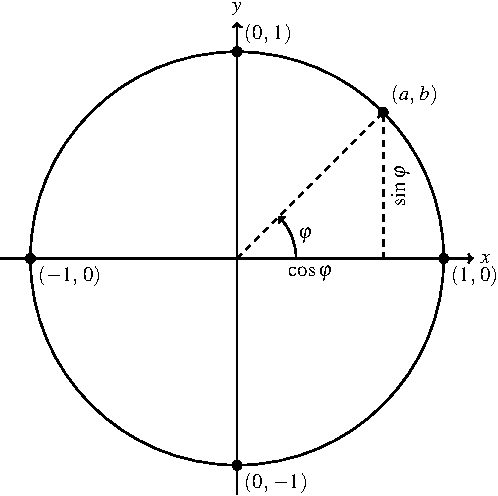
\includegraphics[scale=1.1]{image/04/unit-circle.pdf}
\caption{%%
  A unit circle in the Cartesian coordinate system.  The circle is
  centred at the origin.  If $\tuple{a}{b}$ is any point on the
  circle, the point makes an angle of $\varphi$ radians going
  anti-clockwise from the positive half of the $x$-axis to the point.
}
\label{fig:point_on_unit_circle}
\end{figure}

The angle of $\varphi$ radians tells you how much of the unit circle
to cover.  An angle of $\varphi = 2\pi$ radians means that you make a
complete trip around the unit circle, going anti-clockwise starting
from the point $\tuple{1}{0}$.  The angle $\varphi = \pi$ radians
means your trip only covers half of the unit circle.  Finally,
$\varphi = \pi / 2$ radians means your trip only covers one-quarter of
the unit circle.

\begin{exercise}
Explain why $\cos\pi = -1$ and $\sin\pi = 0$.
\end{exercise}

\ifbool{showSolution}{
\begin{solution}
The point $\tuple{-1}{0}$ on the unit circle in
\Figure{fig:point_on_unit_circle} makes an angle of $\pi$ radians~(or
\degree{180}) with respect to the positive half of the $x$-axis.  So
you can write $\cos\pi = -1$ and $\sin\pi = 0$.
\end{solution}
}{}

\begin{exercise}
\label{ex:cos_sin_270_degrees}
Explain why $\cos\frac{3\pi}{2} = 0$ and $\sin\frac{3\pi}{2} = -1$.
\end{exercise}

\ifbool{showSolution}{
\begin{solution}
The point $\tuple{0}{-1}$ on the unit circle in
\Figure{fig:point_on_unit_circle} makes an angle of $\frac{3\pi}{2}$
radians~(or $\degree{270}$) with respect to the positive half of the
$x$-axis.  So you can write $\cos\frac{3\pi}{2} = 0$ and
$\sin\frac{3\pi}{2} = -1$.
\end{solution}
}{}

\begin{exercise}
Explain why $\cos(-\frac{\pi}{2}) = 0$ and
$\sin(-\frac{\pi}{2}) = -1$.
\end{exercise}

\ifbool{showSolution}{
\begin{solution}
Suppose a point $\tuple{a}{b}$ on the unit circle in
\Figure{fig:point_on_unit_circle} makes an angle of $-\pi / 2$
radians.  The angle is obtained by going clockwise from the positive
half of the $x$-axis to the point $\tuple{a}{b}$.  So going by
$-\pi / 2$ radians is the same as going by $\pi / 2$ radians clockwise
from the positive half of the $x$-axis to $\tuple{a}{b}$.  In other
words, $-\pi / 2$ radians is the same as $\frac{3\pi}{2}$ radians.
Therefore you use the results from \Exercise{ex:cos_sin_270_degrees}
to conclude that $\cos(-\frac{\pi}{2}) = 0$ and
$\sin(-\frac{\pi}{2}) = -1$.
\end{solution}
}{}


%%%%%%%%%%%%%%%%%%%%%%%%%%%%%%%%%%%%%%%%%%%%%%%%%%%%%%%%%%%%%%%%%%%%%%%%%%%

\section{Cartesian to polar}

Let's now discuss how to convert a point $\tuple{a}{b}$ in the
Cartesian coordinate system to the polar coordinate system.
\Figure{fig:convert_from_polar_to_Cartesian_coordinates} illustrates
how the point $\tuple{a}{b}$ can be represented in terms of radius and
angle.  The coordinate system that uses radius and angle is known as
the \emph{polar coordinate system}.  Suppose you want to convert the
Cartesian coordinates $\tuple{a}{b}$ to polar coordinates.  To do so,
you assume that $\tuple{a}{b}$ is a point on a circle that is centred
at the origin.  Then the distance from $\tuple{a}{b}$ to the origin is
the radius of the circle so the radius can be calculated as:
%%
\begin{align*}
r
&=
\sqrt{
  (b - 0)^2 + (a - 0)^2
} \\[4pt]
&=
\sqrt{
  a^2 + b^2
}.
\end{align*}

To calculate the angle $\varphi$ in
\Figure{fig:convert_from_polar_to_Cartesian_coordinates}, you use a
rule called the \emph{law of sines}.  For the triangle in
\Figure{fig:law_of_sines}, the law of sines states that
\[
\frac{a}{\sin\alpha}
=
\frac{b}{\sin\beta}
=
\frac{c}{\sin\gamma}.
\]
This equation is true no matter what the triangle is.  The triangle
can be right-angled, isoceles, or scalene.

\begin{figure}[!htbp]
\centering
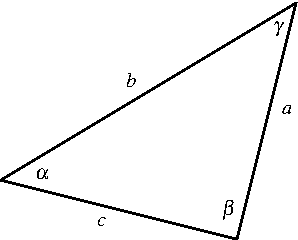
\includegraphics[scale=1.1]{image/04/law-sines.pdf}
\caption{%%
  A triangle with sides $a$, $b$, and $c$.  The angle opposite side
  $a$ is $\alpha$, the angle opposite side $b$ is $\beta$, and the
  angle opposite side $c$ is $\gamma$.
}
\label{fig:law_of_sines}
\end{figure}

From
\Figure{fig:convert_from_polar_to_Cartesian_coordinates} you see that
the dashed vertical line has a length of $b$ and the angle opposite
the radius is $\degree{90}$ or $\pi / 2$ radians.  Use the law of
sines to write
%%
\begin{equation}
\label{eqn:law_of_sines}
\frac{b}{\sin \varphi}
=
\frac{r}{\sin \frac{\pi}{2}}.
\end{equation}
%%
Since $\sin \frac{\pi}{2} = 1$, \Equation{eqn:law_of_sines} can be
simplified to
\[
\frac{b}{\sin \varphi}
=
r.
\]
Solve the last equation for $\sin \varphi$ and you get
$b/r = \sin \varphi$.  Now solve for the angle $\varphi$ and you get
\[
\varphi
=
\arcsin\parenthesis*{\frac{b}{r}}.
\]
The above is summarised as:

\begin{theorem}
\label{thm:convert_Cartesian_to_polar_coordinates}
Let $\tuple{a}{b}$ be a point in the Cartesian coordinate system.
Then $\tuple{a}{b}$ can be written in polar coordinates as
$\tuple{r}{\varphi}$, where
\[
r
=
\sqrt{a^2 + b^2}
%%
\qquad
\text{and}
\qquad
%%
\varphi
=
\arcsin\parenthesis*{\frac{b}{r}}.
\]
\end{theorem}

\begin{figure}[!htbp]
\centering
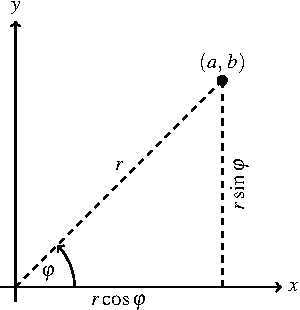
\includegraphics[scale=1.1]{image/04/polar-cartesian.pdf}
\caption{%%
  Any point $\tuple{a}{b}$ in the Cartesian coordinate system can be
  represented as a point $\tuple{r}{\varphi}$ on a circle.  The circle
  is centred at the origin and has a radius of $r$.  The value of
  $\varphi$ radians measures the angle that spans from the positive
  half of the $x$-axis to the radius of the circle, going
  anti-clockwise.  The pair $\tuple{r}{\varphi}$ is known as the
  \emph{polar coordinates} of $\tuple{a}{b}$.  In other words, the
  Cartesian coordinates $\tuple{a}{b}$ and the polar coordinates
  $\tuple{r}{\varphi}$ both describe the same point.
}
\label{fig:convert_from_polar_to_Cartesian_coordinates}
\end{figure}

Let's put \Theorem{thm:convert_Cartesian_to_polar_coordinates} to some
use.  Any point $\tuple{a}{a}$ in the Cartesian coordinate system
makes an angle of $\degree{45}$~(or $\pi / 4$ radians) with respect to
the positive half of the $x$-axis.  In particular, let's convert the
Cartesian coordinates $(\sqrt{2}\comma \sqrt{2})$ to polar
coordinates.  The radius $r$ is
%%
\begin{align*}
r
&=
\sqrt{
  (\sqrt{2})^2 + (\sqrt{2})^2
} \\[4pt]
&=
\sqrt{2 + 2} \\[4pt]
&=
2.
\end{align*}
%%
Since the point $(\sqrt{2}\comma \sqrt{2})$ makes an angle of
$\pi / 4$ radians, then you can write $\varphi$ as
%%
\begin{align*}
\varphi
&=
\arcsin\frac{\sqrt{2}}{2} \\[4pt]
&=
\frac{\pi}{4}.
\end{align*}
%%
Therefore the Cartesian coordinates $(\sqrt{2}\comma \sqrt{2})$ can be
represented as the polar coordinates $(2\comma \frac{\pi}{4})$.

\begin{exercise}
Refer to the unit circle in \Figure{fig:point_on_unit_circle}.
Determine the polar coordinates of each of the Cartesian coordinates
$\tuple{1}{0}$, $\tuple{0}{1}$, $\tuple{-1}{0}$, and $\tuple{0}{-1}$.
\end{exercise}

\ifbool{showSolution}{
\begin{solution}
Each of the points $\tuple{1}{0}$, $\tuple{0}{1}$, $\tuple{-1}{0}$,
and $\tuple{0}{-1}$ lie on the unit circle so in polar coordinates
each of them has a radius of $r = 1$.  The point $\tuple{1}{0}$ makes
an angle of $\varphi = 0$ radians and so $\tuple{1}{0}$ can be written
in polar coordinates as $\tuple{1}{0}$.  The point $\tuple{0}{1}$
makes an angle of $\varphi = \pi / 2$ radians and so it has the polar
representation $(1\comma \frac{\pi}{2})$.  The point $\tuple{-1}{0}$
makes an angle of $\varphi = \pi$ radians and so it can be written as
the polar coordinates $\tuple{1}{\pi}$.  Finally, the point
$\tuple{0}{-1}$ makes an angle of $\varphi = \frac{3\pi}{2}$ radians
and therefore it can be written in polar coordinates as
$(1\comma \frac{3\pi}{2})$.
\end{solution}
}{}


%%%%%%%%%%%%%%%%%%%%%%%%%%%%%%%%%%%%%%%%%%%%%%%%%%%%%%%%%%%%%%%%%%%%%%%%%%%

\section*{Problem}

\begin{problem}
\item Let $n \geq 0$ be an even integer.  Explain why
  $\cos(n\pi) = 1$ and $\sin(n\pi) = 0$.
\ifbool{showSolution}{
  \begin{solution}
  Since $n \geq 0$ is even, it can be written as $n = 2k$ for some
  integer $k \geq 0$.  Then $n\pi = 2k\pi = k(2\pi)$, where $2\pi$
  radians is equivalent to $\degree{360}$.  So $k (2\pi)$ means,
  starting from the point $\tuple{1}{0}$ on the unit circle of
  \Figure{fig:point_on_unit_circle}, you go anti-clockwise $k$ times
  around the unit circle.  One complete trip around the unit circle
  spans $2\pi$ radians, so $k (2\pi)$ radians mean you do $k$ complete
  trips around the unit circle, thus ending up at the point
  $\tuple{1}{0}$.  Therefore $\cos(n\pi) = 1$ and $\sin(n\pi) = 0$.
\end{solution}
}{}

\item Let $n > 0$ be an odd integer.  Explain why $\cos(n\pi) = -1$
  and $\sin(n\pi) = 0$.
\ifbool{showSolution}{
  \begin{solution}
  Since $n > 0$ is odd, it can be written as $n = 2k + 1$ for some
  integer $k \geq 0$.  Note that you can write
  %%
  \begin{align*}
  n\pi
  &=
  (2k + 1) \pi \\[4pt]
  &=
  2k\pi + \pi \\[4pt]
  &=
  k(2\pi) + \pi.
  \end{align*}
  %%
  In other words, starting from the point $\tuple{1}{0}$ on the unit
  circle of \Figure{fig:point_on_unit_circle}, you make $k$ complete
  trips around the unit circle~(going anti-clockwise) and end up at
  the starting point of $\tuple{1}{0}$.  Finally, you go
  anti-clockwise from $\tuple{1}{0}$ by $\pi$ radians.  Your
  destination is now the point $\tuple{-1}{0}$ and therefore
  $\cos(n\pi) = -1$ and $\sin(n\pi) = 0$.
  \end{solution}
}{}

\item Explain why
  $\cos\frac{\pi}{4} = \sin\frac{\pi}{4} = \sqrt{2} / 2$.
\ifbool{showSolution}{
  \begin{solution}
  The point $(\frac{\sqrt{2}}{2}\comma \frac{\sqrt{2}}{2})$ in the
  Cartesian coordinate system makes an angle of
  $\degree{45}$~(or $\varphi = \pi / 4$ radians) with the positive
  half of the $x$-axis.  The distance from the point to the origin is
  %%
  \begin{align*}
  r
  &=
  \sqrt{
    \parenthesis*{\frac{\sqrt{2}}{2}}^2
    +
    \parenthesis*{\frac{\sqrt{2}}{2}}^2
  } \\[4pt]
  &=
  \sqrt{
    \frac{2}{4}
    +
    \frac{2}{4}
  } \\[4pt]
  &=
  1
  \end{align*}
  %%
  and so the point $(\frac{\sqrt{2}}{2}\comma \frac{\sqrt{2}}{2})$
  lies on the unit circle.  Now use
  \Equation{eqn:value_of_x_y_on_unit_circle} to write
  $\sqrt{2} / 2 = \cos\frac{\pi}{4}$ and
  $\sqrt{2} / 2 = \sin\frac{\pi}{4}$, which can also be written as
  $\cos\frac{\pi}{4} = \sin\frac{\pi}{4} = \sqrt{2} / 2$.
  \end{solution}
}{}

\item For which values of $\varphi$ do you have
  $\cos\varphi = -\sqrt{2} / 2$ and $\sin\varphi = \sqrt{2} / 2$?
\ifbool{showSolution}{
  \begin{solution}
  The point $(-\frac{\sqrt{2}}{2}\comma \frac{\sqrt{2}}{2})$ is a
  reflection of the point
  $(\frac{\sqrt{2}}{2}\comma \frac{\sqrt{2}}{2})$ along the $y$-axis.
  So the point $(-\frac{\sqrt{2}}{2}\comma \frac{\sqrt{2}}{2})$ makes
  an angle of $\frac{\pi}{2} + \frac{\pi}{4} = \frac{3\pi}{4}$ radians
  with respect to the positive half of the $x$-axis.  In other words,
  you can write $\cos\frac{3\pi}{4} = -\sqrt{2} / 2$ and
  $\sin\frac{3\pi}{4} = \sqrt{2} / 2$.  Note that if $k \geq 0$ is an
  integer, then you can also write
  \[
  \frac{3\pi}{4} + 2k\pi
  =
  \frac{3\pi}{4}
  \]
  because $2k\pi$ radians is the same as making $k$ complete trips
  around the unit circle.  After those $k$ complete trips, you end up
  where you started on the unit circle.  Therefore if $k \geq 0$ is an
  integer and you have
  \[
  \varphi
  =
  \frac{3\pi}{4} + 2k\pi
  \]
  then $\cos\varphi = -\sqrt{2} / 2$ and $\sin\varphi = \sqrt{2} / 2$.
  \end{solution}
}{}
\end{problem}

\end{document}
